\documentclass[11pt,letterpaper]{article}

% ---------- Packages ----------
\usepackage[T1]{fontenc}
\usepackage[utf8]{inputenc}
\usepackage{lmodern}
\usepackage[margin=1in]{geometry}
\usepackage{amsmath,amssymb}
\usepackage{siunitx}
\sisetup{detect-all, group-separator={,}, group-minimum-digits=4}
\usepackage{booktabs}
\usepackage{array}
\usepackage{graphicx}
\usepackage{caption}
\usepackage{subcaption}
\usepackage{float}
\usepackage{enumitem}
\usepackage{xcolor}
\usepackage{tikz}
\usetikzlibrary{arrows.meta,positioning,shapes.geometric}
\usepackage{pgfplots}
\pgfplotsset{compat=1.17}
\usepackage{listings}
\usepackage{xurl}
\usepackage[hidelinks]{hyperref}

\captionsetup{font=small,labelfont=bf}
\setlist{itemsep=2pt,topsep=4pt}

\definecolor{codegray}{gray}{0.45}
\definecolor{pvblue}{HTML}{2A6FDB}
\definecolor{accent}{HTML}{C2410C}
\lstset{
  language=Python,
  basicstyle=\ttfamily\scriptsize,
  numbers=left, numberstyle=\tiny\color{codegray}, numbersep=6pt,
  keywordstyle=\color{blue!60!black}\bfseries,
  commentstyle=\color{green!40!black}\itshape,
  stringstyle=\color{red!55!black},
  breaklines=true, breakatwhitespace=true,
  showstringspaces=false, columns=fullflexible, keepspaces=true,
  frame=none, xleftmargin=1.5em
}

\newcommand{\pu}{\,\mathrm{pu}}

% ---------- Title ----------
\title{\textbf{PV Hosting Capacity and DER Interconnection\\Study of the IEEE 34-Bus Test Feeder}\\[6pt]
\large Full-Year Time-Series Analysis with IEEE 1547-2018 Smart Inverter Functions,\\
a Fault Study and Interconnection Screens}
\author{Mahedi Hasan\\[2pt]
\normalsize Department of Electrical Engineering, The City College of New York}
\date{November 15, 2026}

\begin{document}
\maketitle

\begin{abstract}
\noindent
This report describes a distributed energy resource (DER) interconnection study of the IEEE 34-node test
feeder, a long, lightly loaded \SI{24.9}{kV} rural feeder in Arizona. The feeder was modeled in OpenDSS and
driven from Python through OpenDSSDirect.py. The model was first validated against IEEE's published power
flow: with regulator taps matched, all 92 bus-phase voltages agreed within \textbf{0.14\,\%} (mean
0.06\,\%) and substation power within 0.6\,\%. A full-year, hourly (8{,}760\,h) time-series simulation was then
run with a utility load shape and NSRDB solar data for Tucson, AZ, sweeping the size of a PV plant at bus 848
in \SI{50}{kW} steps against the ANSI C84.1 Range A limit of \SI{1.05}{pu} and conductor thermal ratings.
The hosting capacity was \textbf{800\,kW at unity power factor}, \textbf{900\,kW with IEEE 1547-2018
Category B volt-var} and 1{,}050\,kW at a fixed 0.95 power factor (absorbing). Every case was limited by
overvoltage at bus 814, the end of the 20-mile unregulated section ahead of the first line regulator, and a
simple $\Delta V \approx (PR-QX)/V^2$ estimate predicted the measured voltage slope within 4\,\% and the gain from
reactive power within 1\,\%. Lowering the substation setpoint from IEEE's \SI{1.05}{pu} to \SI{1.03}{pu}
raised hosting capacity eightfold (100 to 800\,kW), but a fixed 1.03\,pu setting lowers bus 814 below
0.95\,pu for 296 hours a year at heavy load (14 hours at 1.05\,pu), so in practice the setpoint would have to follow
the load. A fault study showed the PV adds at most 13\,\% to the
end-of-line fault current, and all sizes fail the 10\,\% fault-current and 15\,\%-of-peak-load fast-track screens,
showing why detailed studies are needed on long feeders.
\end{abstract}

\tableofcontents
\newpage

% =====================================================================
\section{Introduction}
Rooftop and community solar are being connected to distribution feeders faster than utilities can study
them one by one. Before a PV system is approved, the utility asks two questions: will the feeder stay within
voltage and thermal limits in every hour of the year, and will the new generation upset protection? The
largest PV size that passes these tests without grid upgrades is the feeder's \emph{hosting capacity}.

The goals of this project were to:
\begin{enumerate}
  \item build and validate an OpenDSS model of the IEEE 34-bus feeder against IEEE's published results;
  \item find the PV hosting capacity at the end of the feeder with a full-year, hourly time-series simulation;
  \item compare unity power factor with the IEEE 1547-2018 volt-var and constant power factor functions;
  \item run a fault study with and without PV and apply standard fast-track interconnection screens;
  \item keep the whole study reproducible: every number in this report is produced by a script in the
        project's public GitHub repository.
\end{enumerate}

% =====================================================================
\section{Theory}

\subsection{Voltage rise from distributed generation}
For a short line with resistance $R$ and reactance $X$ carrying real power $P$ and reactive power $Q$
\emph{away} from a source of voltage $V$, the voltage change along the line is approximately
\begin{equation}
  \frac{\Delta V}{V} \approx \frac{P R + Q X}{V^2}.
  \label{eq:dv}
\end{equation}
A PV plant that exports power reverses $P$, so the voltage at its end of the line \emph{rises}. If the
inverter absorbs reactive power ($Q<0$ in the generator convention), the $QX$ term opposes the $PR$ term:
\begin{equation}
  \frac{\Delta V}{V} \approx \frac{P R}{V^2}\left(1 - \frac{|Q|}{P}\,\frac{X}{R}\right).
  \label{eq:dvq}
\end{equation}
Equation~\eqref{eq:dvq} shows that reactive power absorption helps most on lines with a high $X/R$ ratio,
and that the benefit scales with $|Q|/P$. If the limit is a fixed voltage rise, the hosting capacity grows by
the factor $1/(1-(|Q|/P)(X/R))$. This is used in Section~\ref{sec:theorycheck} as an independent check.

\subsection{Step voltage regulators}
A step voltage regulator is an autotransformer with 32 taps of 0.625\,\% each ($\pm10$\,\%). It holds the voltage
at its output, or at a point downstream through line-drop compensation (LDC), inside a bandwidth around a
setpoint. The IEEE 34-bus regulators use a 2\,V bandwidth on a 120\,V base ($\pm 1$\,V). Two consequences
matter for this study:
\begin{itemize}
  \item more than one tap position can satisfy the bandwidth, so two correct programs can settle on
        different taps;
  \item a regulator controls only its \emph{output} side. The section between the substation and the first
        regulator is set only by the substation voltage.
\end{itemize}

\subsection{Voltage limits}
ANSI C84.1 Range A requires service voltage to stay within $\pm5$\,\% of nominal under normal conditions.
This study uses 0.95--1.05\,pu on every primary node. Because PV raises voltage, only the upper limit can be
newly violated by PV.

\subsection{IEEE 1547-2018 reactive power functions}
\paragraph{Constant power factor.} The inverter keeps a fixed ratio of reactive to real power,
\begin{equation}
  |Q| = P \tan\!\left(\cos^{-1}\mathrm{PF}\right), \qquad \mathrm{PF}=0.95 \Rightarrow |Q| = 0.329\,P.
\end{equation}
\paragraph{Volt-var.} The inverter sets $Q$ from its \emph{local terminal voltage} along a piecewise-linear
curve. The Category B default curve (Fig.~\ref{fig:vvcurve}) supplies up to 44\,\% of rated kVA as vars at
0.92\,pu and below, does nothing in the 0.98--1.02\,pu deadband, and absorbs up to 44\,\% at 1.08\,pu and above.
To deliver 44\,\% vars at full real output, the inverter kVA must satisfy $S^2 = P^2 + (0.44S)^2$, so
$S = P/\sqrt{1-0.44^2} = 1.114\,P$; a ratio of 1.12 was used.

\begin{figure}[H]
\centering
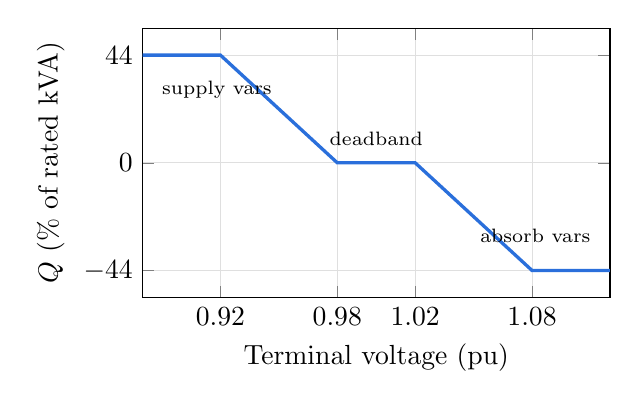
\begin{tikzpicture}
\begin{axis}[
  width=0.62\textwidth, height=5cm,
  xlabel={Terminal voltage (pu)}, ylabel={$Q$ (\% of rated kVA)},
  xmin=0.88, xmax=1.12, ymin=-55, ymax=55,
  xtick={0.92,0.98,1.02,1.08}, ytick={-44,0,44},
  grid=major, grid style={gray!25},
  every axis plot/.append style={very thick}
]
\addplot[pvblue] coordinates {(0.88,44) (0.92,44) (0.98,0) (1.02,0) (1.08,-44) (1.12,-44)};
\node[font=\scriptsize, anchor=west] at (axis cs:0.885,30) {supply vars};
\node[font=\scriptsize, anchor=east] at (axis cs:1.115,-30) {absorb vars};
\node[font=\scriptsize] at (axis cs:1.0,10) {deadband};
\end{axis}
\end{tikzpicture}
\caption{IEEE 1547-2018 Category B default volt-var curve used in this study.}
\label{fig:vvcurve}
\end{figure}

\subsection{Hosting capacity}
Hosting capacity is the largest DER size that can be connected at a location with no limit violated in any
hour studied and no upgrades. Here the limits are overvoltage ($V>1.05$\,pu) on any primary node and loading
above 100\,\% of the normal rating of any line or transformer.

\subsection{Inverter fault current and interconnection screens}
Rotating generators can supply 5--10 times rated current into a fault; inverters are limited by their
electronics to roughly 1.1--1.5 times rated. Many utilities use fast-track \emph{screens} before a detailed
study. Arizona Admin.\ Code R14-2-2615, which follows the FERC Small Generator Interconnection Procedures
(SGIP), includes:
\begin{itemize}
  \item aggregate generation on the circuit $\le 15$\,\% of the circuit's annual peak load;
  \item the proposed generation must not add more than 10\,\% to the circuit's maximum fault current.
\end{itemize}
A project that fails a screen is not rejected; it goes to supplemental review or a detailed study such as
this one.

% =====================================================================
\section{Feeder Model}

\subsection{The IEEE 34-node test feeder}
The feeder (Fig.~\ref{fig:oneline}) is an actual \SI{24.9}{kV} feeder in Arizona, published by the IEEE PES
Distribution Test Feeder Working Group. It is long and lightly loaded, so voltage regulation dominates its
behavior.

\begin{figure}[H]
\centering
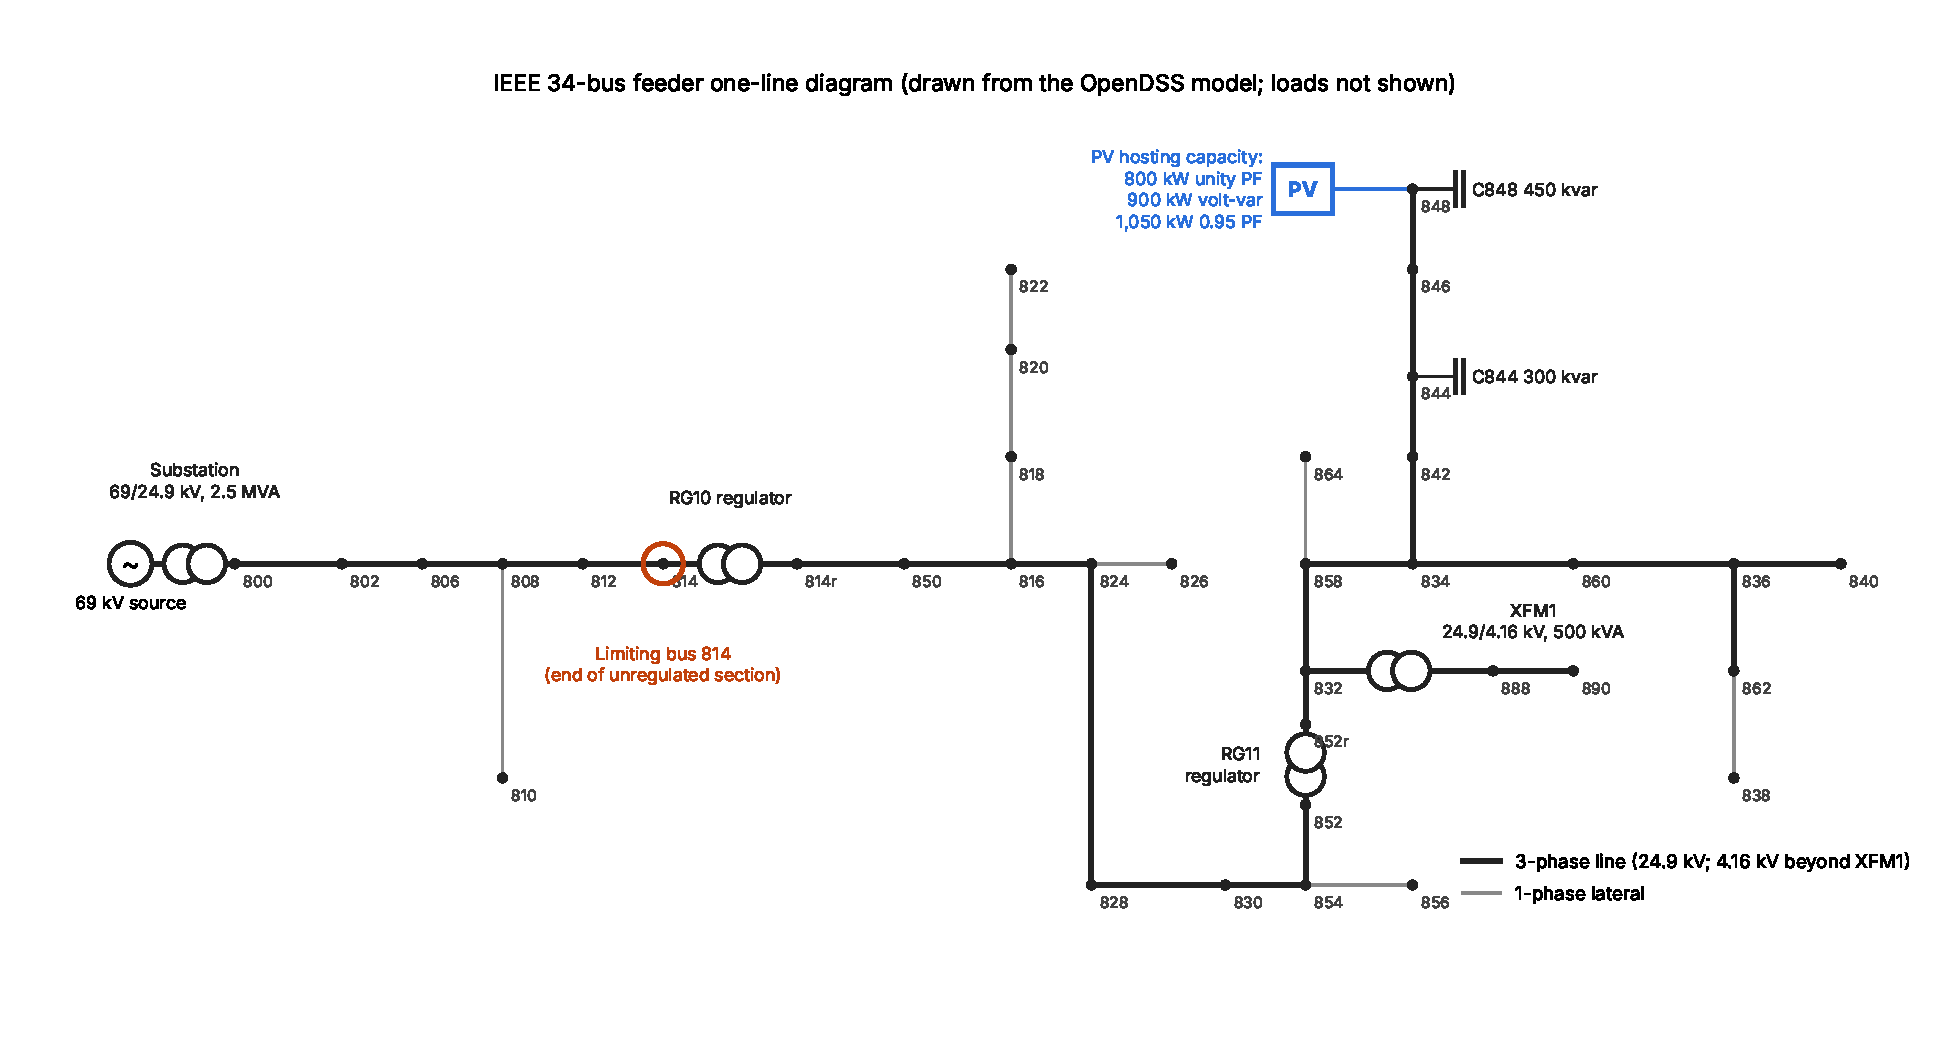
\includegraphics[width=\textwidth]{figures/fig_step6_one_line.pdf}
\caption{One-line diagram drawn directly from the OpenDSS model by \texttt{one\_line.py}. The PV plant is at
bus 848; the limiting bus 814 is circled. Loads are not shown.}
\label{fig:oneline}
\end{figure}

\begin{table}[H]
\centering
\small
\begin{tabular}{@{}ll@{}}
\toprule
Item & Value \\
\midrule
Nominal voltage & \SI{24.9}{kV} primary; \SI{4.16}{kV} beyond XFM1 \\
Line length & 58.4\,mi total (33 segments, \num{308114}\,ft); farthest bus (838) 36.7\,mi from substation \\
Load & \SI{1769}{kW} nameplate (spot and distributed, Y and $\Delta$, constant $PQ$/$I$/$Z$) \\
Regulators & RG10 at 814 (122\,V, $R$=2.7, $X$=1.6); RG11 at 852 (124\,V, $R$=2.5, $X$=1.5) \\
Capacitors & C844 300\,kvar, C848 450\,kvar (fixed) \\
Transformers & Substation 69/24.9\,kV 2.5\,MVA; XFM1 24.9/4.16\,kV 500\,kVA \\
Conductors & Config.\ 300: 1/0 ACSR; 301, 304: \#2 ACSR; 302, 303: \#4 ACSR \\
\bottomrule
\end{tabular}
\caption{Main feeder data.}
\label{tab:feeder}
\end{table}

\subsection{Tools}
\begin{table}[H]
\centering
\small
\begin{tabular}{@{}ll@{}}
\toprule
Tool / data & Version and role \\
\midrule
OpenDSS model & EPRI \texttt{ieee34Mod1.dss}, shipped with OpenDSS 11.0.0.1 \\
Solver interface & OpenDSSDirect.py 0.9.4 (DSS C-API 0.14.5, based on OpenDSS SVN 3723) \\
Language & Python 3.12 (virtual environment), pandas, NumPy, matplotlib \\
Load profile & EPRI \texttt{PaperLoadShape.txt}, 8{,}760 hourly multipliers \\
PV profile & PVWatts V8 (NSRDB TMY), Tucson, AZ \\
Version control & Git, public GitHub repository \texttt{mhasan-ee/ieee34-hosting-capacity} \\
\bottomrule
\end{tabular}
\caption{Software and data.}
\end{table}

\subsection{Line ratings}
The IEEE model leaves every line at OpenDSS's default normal rating of 400\,A, which is a placeholder. Standard
ACSR ampacities were assigned by line code: 1/0 ACSR \SI{230}{A}, \#2 ACSR \SI{180}{A}, \#4 ACSR \SI{140}{A}
(Kersting, Appendix~A).

% =====================================================================
\section{Study Workflow}
Each step of the study is a separate script that writes its results to CSV files and figures
(Fig.~\ref{fig:workflow}). The full commands are in Appendix~\ref{app:run}.

\begin{figure}[H]
\centering
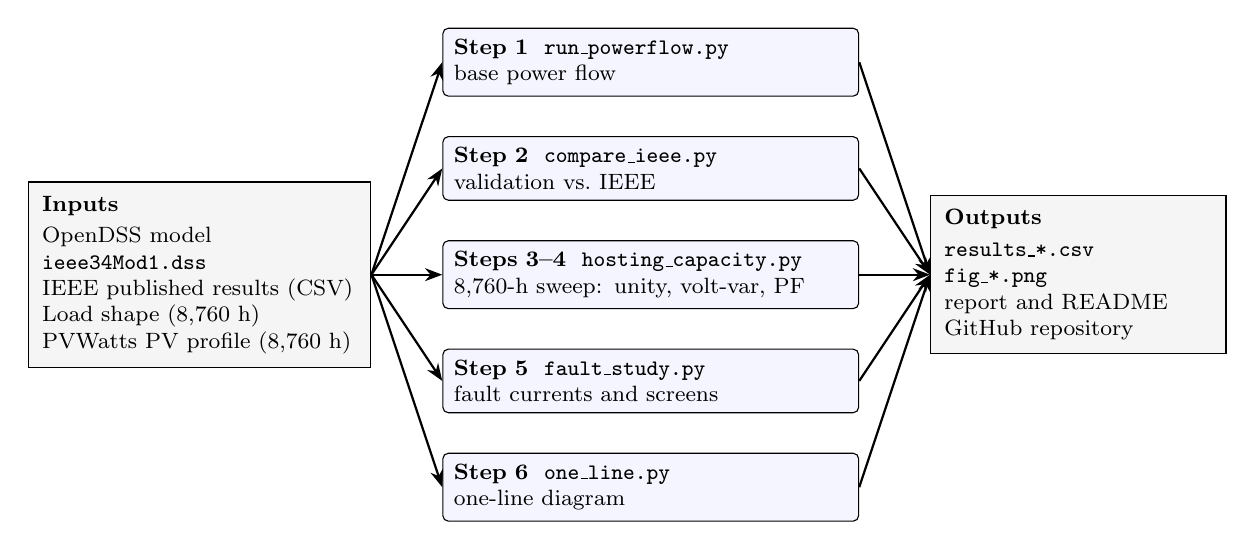
\begin{tikzpicture}[
  node distance=5mm and 9mm,
  data/.style={draw, align=left, font=\footnotesize, text width=40mm, fill=gray!8, inner sep=5pt},
  box/.style={draw, rounded corners=2pt, align=left, font=\footnotesize, text width=50mm, fill=blue!4, inner sep=4pt},
  arr/.style={-{Stealth[length=2.2mm]}, thick}
]
\node[box] (s1) {\textbf{Step 1} \ \texttt{run\_powerflow.py}\\ base power flow};
\node[box, below=of s1] (s2) {\textbf{Step 2} \ \texttt{compare\_ieee.py}\\ validation vs.\ IEEE};
\node[box, below=of s2] (s3) {\textbf{Steps 3--4} \ \texttt{hosting\_capacity.py}\\ 8{,}760-h sweep: unity, volt-var, PF};
\node[box, below=of s3] (s5) {\textbf{Step 5} \ \texttt{fault\_study.py}\\ fault currents and screens};
\node[box, below=of s5] (s6) {\textbf{Step 6} \ \texttt{one\_line.py}\\ one-line diagram};
\node[data, left=of s3] (in) {\textbf{Inputs}\\[2pt]
  OpenDSS model \texttt{ieee34Mod1.dss}\\ IEEE published results (CSV)\\ Load shape (8{,}760 h)\\ PVWatts PV profile (8{,}760 h)};
\node[data, right=of s3, text width=34mm] (out) {\textbf{Outputs}\\[2pt]
  \texttt{results\_*.csv}\\ \texttt{fig\_*.png}\\ report and README\\ GitHub repository};
\foreach \n in {s1,s2,s3,s5,s6} {\draw[arr] (in.east) -- (\n.west);}
\foreach \n in {s1,s2,s3,s5,s6} {\draw[arr] (\n.east) -- (out.west);}
\end{tikzpicture}
\caption{Study workflow. Grey blocks are data; blue blocks are scripts.}
\label{fig:workflow}
\end{figure}

% =====================================================================
\section{Model Validation}

\subsection{First power flow}
The base case solved in 25 iterations (including regulator control iterations) with 37 buses. The substation
supplied \SI{2047.0}{kW} and \SI{283.3}{kvar}; losses were \SI{273.5}{kW} (13.4\,\% of input), high but expected
on a feeder this long.

\subsection{Comparison with IEEE published results}
IEEE's published power flow (Kersting) was extracted from the IEEE document into a CSV of 95 bus-phase voltages
with angles and distances. IEEE's regulator output nodes RG10/RG11 correspond to OpenDSS buses 814r/852r, and
the in-line node XF10 has no separate OpenDSS bus, leaving 92 comparable voltages.

\begin{table}[H]
\centering
\small
\begin{tabular}{@{}lrrr@{}}
\toprule
Quantity & OpenDSS, auto taps & OpenDSS, IEEE taps & IEEE published \\
\midrule
Substation kW & 2047.0 (+0.20\,\%) & 2030.8 ($-$0.59\,\%) & 2042.9 \\
Substation kvar & 283.3 ($-$2.40\,\%) & 284.5 ($-$1.97\,\%) & 290.3 \\
Losses kW & 273.5 (+0.17\,\%) & 270.1 ($-$1.08\,\%) & 273.0 \\
Mean $|$voltage error$|$ & 0.58\,\% & \textbf{0.06\,\%} & -- \\
Max $|$voltage error$|$ & 1.36\,\% (890 A) & \textbf{0.14\,\%} (890 B) & -- \\
Voltages within 1\,\% & 66 / 92 & 92 / 92 & -- \\
RG10 taps A/B/C & +14 / +4 / +5 & +12 / +5 / +5 & +12 / +5 / +5 \\
RG11 taps A/B/C & +13 / +13 / +13 & +13 / +11 / +12 & +13 / +11 / +12 \\
\bottomrule
\end{tabular}
\caption{OpenDSS vs.\ IEEE published power flow.}
\label{tab:validation}
\end{table}

\begin{figure}[H]
\centering
\begin{subfigure}{0.49\textwidth}
  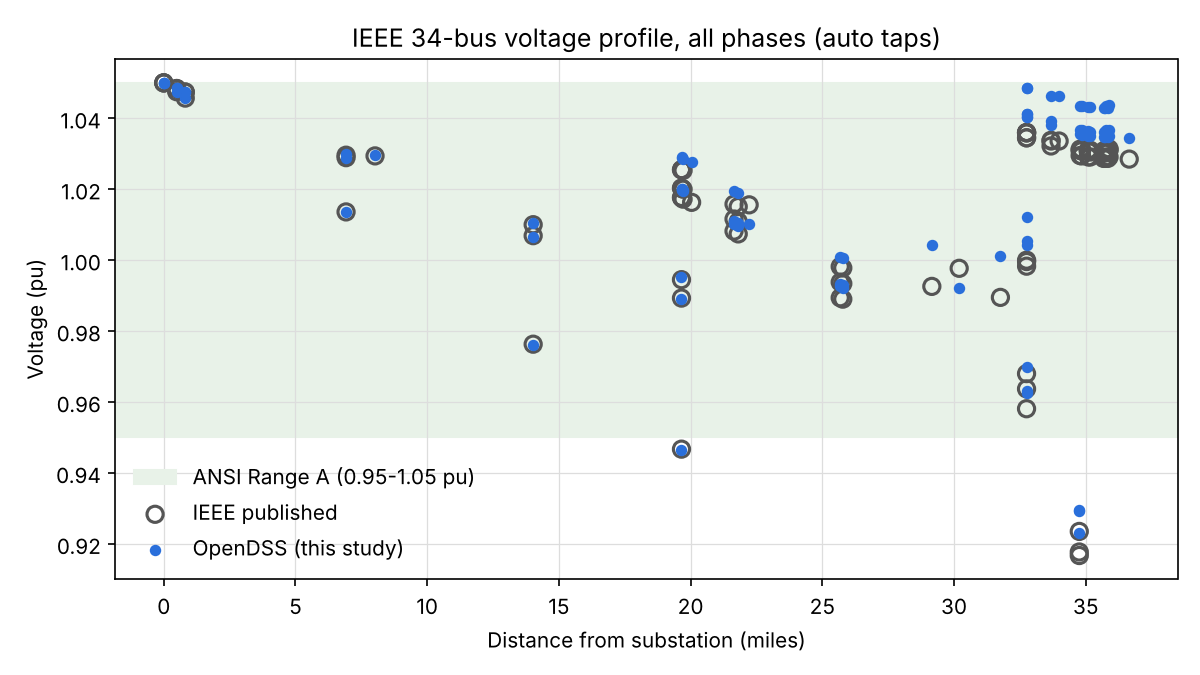
\includegraphics[width=\linewidth]{figures/fig_step2_profile_auto_taps.png}
  \caption{OpenDSS chooses its own taps}
\end{subfigure}\hfill
\begin{subfigure}{0.49\textwidth}
  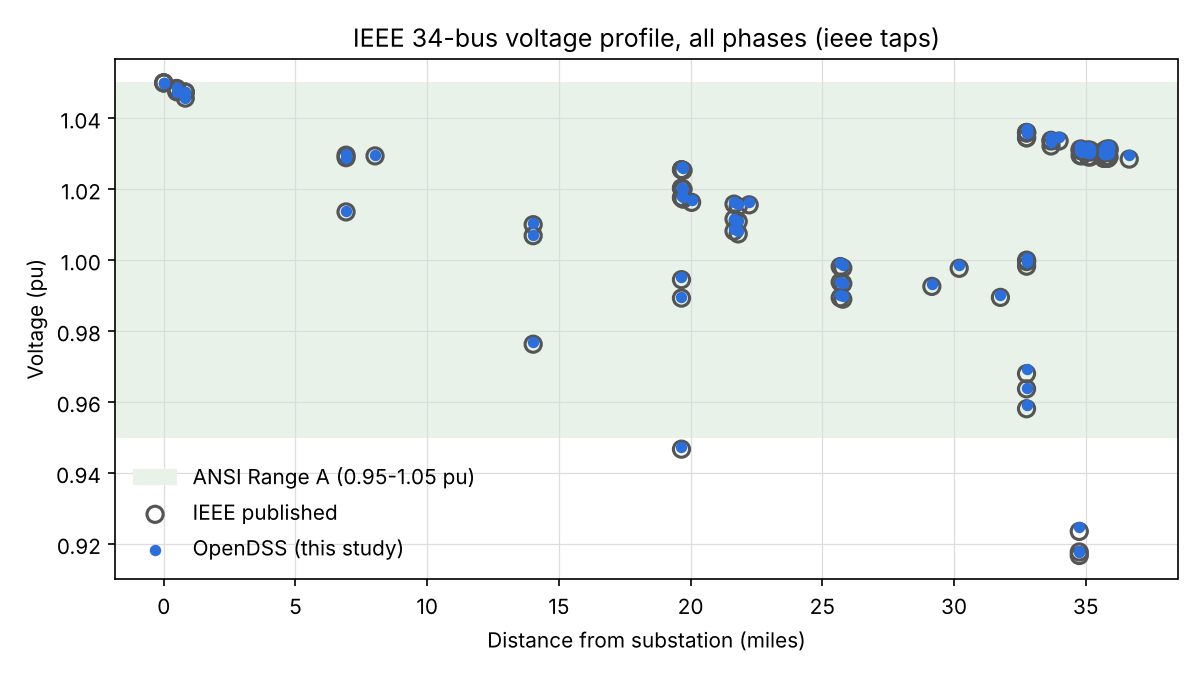
\includegraphics[width=\linewidth]{figures/fig_step2_profile_ieee_taps.png}
  \caption{Taps locked at IEEE's values}
\end{subfigure}
\caption{Voltage profile of all phases: OpenDSS (dots) vs.\ IEEE published (rings). The green band is ANSI
Range A.}
\label{fig:profiles2}
\end{figure}

\subsection{Discussion}
With OpenDSS choosing its own taps, buses upstream of RG10 matched IEEE almost exactly, but phase A downstream
read about 1.2\,\% high. RG10 phase A had settled two taps higher than IEEE's program
($2\times0.625\,\%=1.25\,\%$), which explains the offset exactly. Both tap sets lie inside the 2\,V bandwidth,
so both are valid. With the taps locked at IEEE's values the voltages agree within 0.14\,\%, which
validates the line, load and transformer models. The remaining 0.6\,\% gap in substation power most likely
comes from how the two programs place distributed loads along each segment; voltage-dependent loads also
draw slightly less power at the lower phase-A voltage.

% =====================================================================
\section{Load and Solar Profiles}
The EPRI load shape has a minimum of 0.266, a mean (load factor) of 0.537 and its peak on Aug 10 at
2\,PM; its minimum is at 11\,PM on Oct 16, when PV produces nothing. PVWatts V8 was run for Tucson, AZ
(NSRDB 32.21$^\circ$N, 110.98$^\circ$W) with the default \SI{4}{kW} system (fixed, 20$^\circ$ tilt, south facing,
14.08\,\% losses, DC/AC ratio 1.2). It produced \SI{7150}{kWh} per year, or \SI{1788}{kWh/kW_{dc}}, an AC
capacity factor of 24.5\,\%. Output was normalized to the inverter AC rating, so the profile is 0--1\,pu;
the inverter clipped in only 6 hours. May is the best month because the July--August monsoon clouds reduce
summer output.

\begin{figure}[H]
\centering
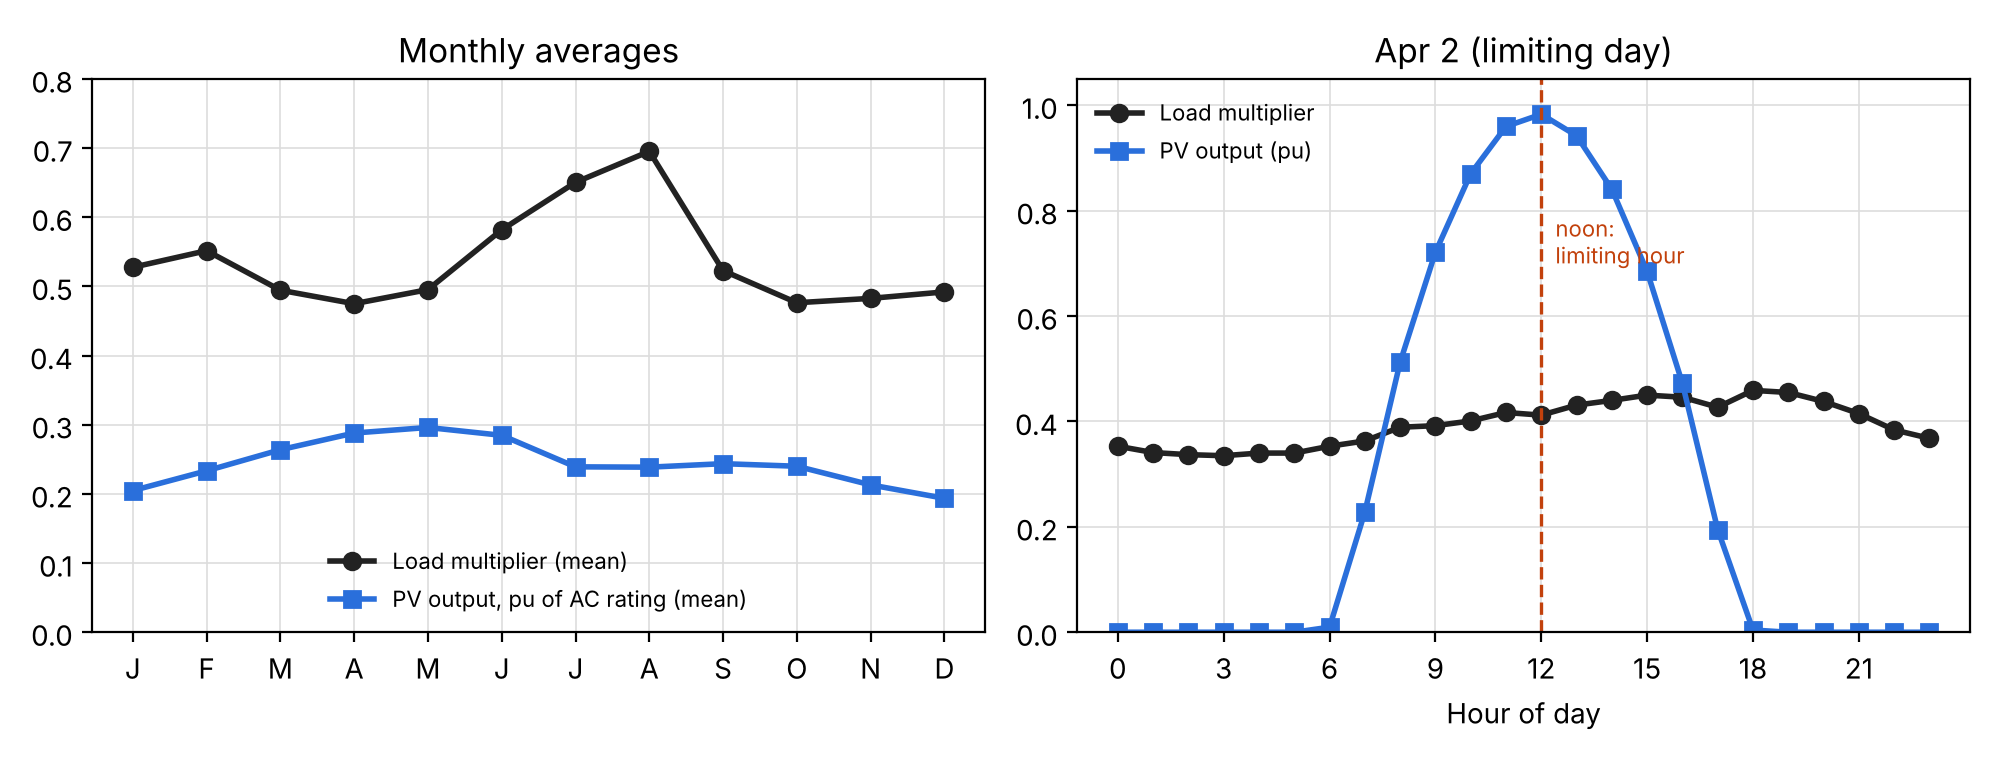
\includegraphics[width=\textwidth]{figures/fig_report_profiles.png}
\caption{Input profiles. Left: monthly averages. Right: Apr 2, the day that limits hosting capacity: at noon
PV is at 0.983\,pu while load is only 0.412 of peak.}
\label{fig:inputprofiles}
\end{figure}

The critical condition for overvoltage is not the minimum load of the year but the lowest load
\emph{during strong sun}: mild spring and autumn middays, as Fig.~\ref{fig:inputprofiles} shows.

% =====================================================================
\section{Hosting Capacity}

\subsection{Method}
\begin{enumerate}
  \item A three-phase PV system (OpenDSS \texttt{PVSystem}) is placed at bus 848, the end of the 3-phase
        \SI{24.9}{kV} trunk.
  \item For each PV size from 0\,kW upward in 50\,kW steps, all 4{,}264 daylight hours are solved. Each hour
        sets the global load multiplier from the load shape and the PV irradiance from the PV profile.
        Night hours are skipped because PV cannot cause violations without output.
  \item Regulators act in each snapshot (static control). The highest node voltage and the highest line
        or transformer loading over the year are recorded, with the hour and location.
  \item The first size that violates a limit ends the sweep; the largest passing size is the hosting
        capacity. A 0.0001\,pu tolerance removes floating-point round-off.
  \item Undervoltages are excluded from the hosting capacity check, because PV cannot make them worse.
        They are reported separately in Section~\ref{sec:setpoint} (bus 814 phase A and the 4.16\,kV bus 890
        at peak load).
  \item Every one of the 4{,}264 hourly solutions converged in every run.
\end{enumerate}

\subsection{Choice of substation setpoint}\label{sec:setpoint}
IEEE fixes the source at 1.05\,pu, a peak-load setting. At the lightest-load hour of the year (11\,PM, Oct 16)
this alone puts bus 814 above the limit with no PV at all (Table~\ref{tab:source}). The study therefore uses
1.03\,pu, a typical substation LTC setpoint.

This choice has a cost. Bus 814 is on the source side of RG10, so only the substation sets its voltage:
lowering the source by 0.02\,pu lowers bus 814 by about the same amount in every hour. At peak load, phase A
at bus 814 drops from 0.946\,pu to 0.924\,pu, and over the whole year bus 814 is below 0.95\,pu for 296 hours
instead of 14. Buses beyond the line regulators are barely affected, because RG10 and RG11 raise their taps
to compensate. A single fixed setpoint therefore cannot keep this feeder inside Range A at both light and
heavy load. In practice the substation LTC would raise its voltage with load (line-drop compensation or a
load-dependent schedule). That would remove most of the undervoltage hours, but it would also lower the
hosting capacity found here, because the limiting hours (spring middays at about 40\,\% load) would see a
slightly higher sending voltage. The 1.03\,pu results below are therefore the hosting capacity for that
setpoint, not a final operating recommendation.

\begin{table}[H]
\centering
\small
\begin{tabular}{@{}lcccc@{}}
\toprule
Source & Light load (hr 6935) & Peak load (hr 5318) & Bus 814 A & Hours/yr with \\
setting & max $V$ (pu) & min $V$ (pu) & at peak (pu) & 814 $<0.95$\,pu \\
\midrule
1.05\,pu (IEEE) & \textbf{1.0528 at 814.2} & 0.9231 at 890.3 & 0.946 & 14 \\
1.03\,pu (this study) & 1.0328 at 814.2 & 0.9241 at 814.1 & \textbf{0.924} & \textbf{296} \\
\bottomrule
\end{tabular}
\caption{Effect of the substation setpoint with no PV, over all 8{,}760 hours (\texttt{setpoint\_check.py}).}
\label{tab:source}
\end{table}

\subsection{Results}
\begin{table}[H]
\centering
\small
\begin{tabular}{@{}lrrll@{}}
\toprule
Case (PV at bus 848) & Hosting capacity & First fail & Limiting voltage & When \\
\midrule
Unity PF, 1.05\,pu source (IEEE) & 100\,kW & 150\,kW & 1.0504\,pu at 814.2 & Nov 23, 1\,PM \\
Unity PF, 1.03\,pu source & \textbf{800\,kW} & 850\,kW & 1.0510\,pu at 814.3 & Apr 2, noon \\
Volt-var, IEEE 1547 Cat B & \textbf{900\,kW} & 950\,kW & 1.0501\,pu at 814.3 & Apr 9, noon \\
Constant 0.95 PF, absorbing & \textbf{1{,}050\,kW} & 1{,}100\,kW & 1.0505\,pu at 814.3 & Apr 2, noon \\
\bottomrule
\end{tabular}
\caption{Hosting capacity results (50\,kW resolution, 8{,}760-hour profiles).}
\label{tab:hc}
\end{table}

\begin{figure}[H]
\centering
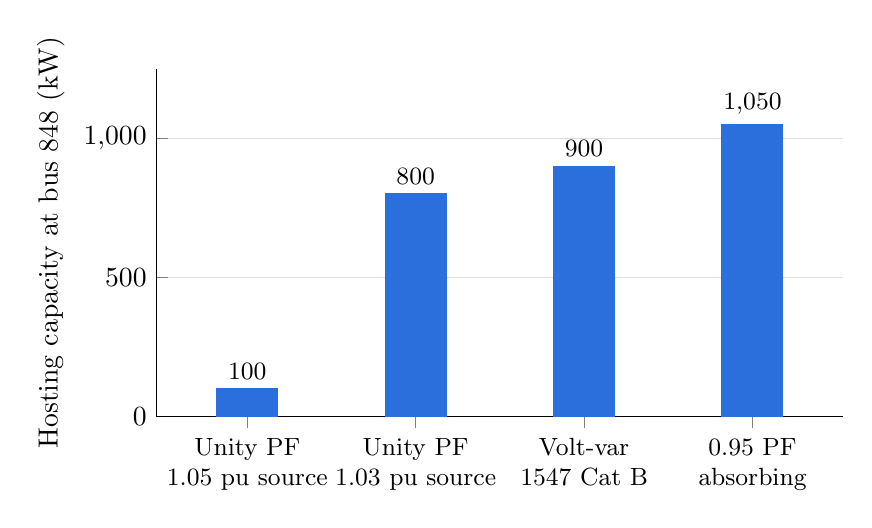
\begin{tikzpicture}
\begin{axis}[
  ybar, bar width=22pt,
  width=0.85\textwidth, height=6cm,
  ymin=0, ymax=1250,
  ylabel={Hosting capacity at bus 848 (kW)},
  symbolic x coords={IEEE1.05, Unity, VV, PF95},
  xticklabels={{Unity PF\\1.05 pu source}, {Unity PF\\1.03 pu source}, {Volt-var\\1547 Cat B}, {0.95 PF\\absorbing}},
  xtick=data, xticklabel style={align=center, font=\small},
  nodes near coords, nodes near coords style={font=\small},
  ymajorgrids, grid style={gray!25},
  enlarge x limits=0.18,
  axis x line*=bottom, axis y line*=left
]
\addplot[fill=pvblue, draw=pvblue] coordinates {(IEEE1.05,100) (Unity,800) (VV,900) (PF95,1050)};
\end{axis}
\end{tikzpicture}
\caption{PV hosting capacity by case.}
\label{fig:hcbar}
\end{figure}

\begin{figure}[H]
\centering
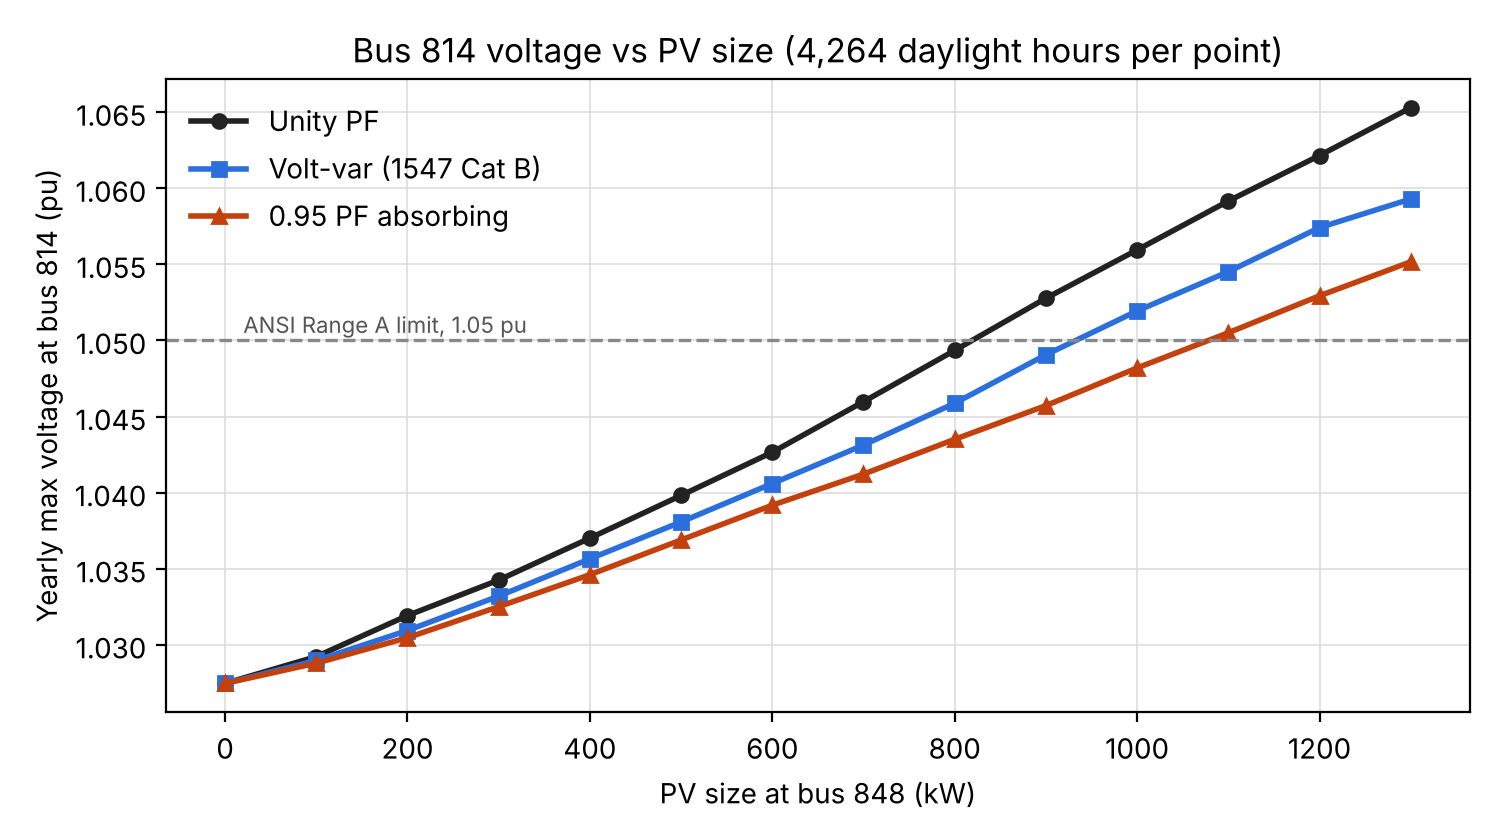
\includegraphics[width=0.85\textwidth]{figures/fig_report_v814.png}
\caption{Yearly maximum voltage at bus 814 vs.\ PV size, 1.03\,pu source. Each point is the highest of
4{,}264 hourly solutions. The PV size where each curve crosses 1.05\,pu is its hosting capacity.}
\label{fig:v814}
\end{figure}

\subsection{Why bus 814 limits}
Below about 800\,kW, the feeder's highest voltage over the year stays at 1.0485--1.0498\,pu at the RG11
output (852r) on summer afternoons. That voltage is set by RG11's line-drop compensation at peak load, not by
PV, so it barely changes with PV size. Above about 800\,kW, midday PV exceeds the downstream load
(at Apr 2 noon the feeder load is $0.412\times1769\approx729$\,kW) and power flows back toward the substation
through both regulators. The regulators lower their taps to protect the buses after them, but bus 814 sits on
the \emph{input} side of RG10 with nothing regulating it, so its voltage rises past 1.05\,pu
(Fig.~\ref{fig:v814}). Thermal limits were never approached: the highest loading in any case was 91.9\,\%
(XFM1, which serves load, not PV), and the PV current at these sizes (20--30\,A at \SI{24.9}{kV}) is far
below the 140--230\,A conductor ratings.

\subsection{Why volt-var helps only a little}
A volt-var inverter reacts to its \emph{own} terminal voltage. RG11 holds bus 848 near 1.03--1.04\,pu, just past
the 1.02\,pu edge of the deadband, so the inverter absorbs only a small share of its capability. At
\SI{900}{kW} on Apr 2 at noon it produced \SI{884.7}{kW} and absorbed \SI{117.2}{kvar} of the \SI{443}{kvar}
available (26\,\%). The problem bus is about 16\,miles upstream behind two regulators, where the inverter cannot
see it. A fixed 0.95 PF absorbs $0.329$\,kvar per kW in every hour regardless of local voltage, so it lowers
the voltage at 814 more, at the cost of higher losses and more reactive power drawn from the substation.

\subsection{Check against theory}
\label{sec:theorycheck}
The section from the substation to bus 814 is 103.77\,kft of configuration 300 (1/0 ACSR). Averaging the
self and mutual terms of its impedance matrix gives the positive-sequence impedance
\[
  R_1 = 0.2519-0.0398 = 0.2121\ \Omega/\text{kft}, \quad
  X_1 = 0.2549-0.0971 = 0.1578\ \Omega/\text{kft}, \quad X/R = 0.744,
\]
so $Z_1 = 22.01 + j16.38\ \Omega$. By Eq.~\eqref{eq:dv}, each 100\,kW of reverse power at unity PF raises bus
814 by
\[
  \frac{\Delta V}{V} \approx \frac{100\times10^3 \times 22.01}{(24.9\times10^3)^2} = 0.00355\ \text{pu}.
\]
The simulated slope between 700 and 900\,kW is $(1.0528-1.0460)/2 = 0.0034$\,pu per 100\,kW, within 4\,\%.

Equation~\eqref{eq:dvq} predicts the gain from reactive power:

\begin{table}[H]
\centering
\small
\begin{tabular}{@{}lcccc@{}}
\toprule
Mode & $|Q|/P$ & Predicted gain & Predicted HC & Simulated HC \\
\midrule
0.95 PF absorbing & 0.329 & 1.324 & $800\times1.324 = 1059$\,kW & 1050\,kW ($-$0.8\,\%) \\
Volt-var (Apr 2 noon) & 0.132 & 1.109 & $800\times1.109 = 887$\,kW & 900\,kW (+1.4\,\%) \\
\bottomrule
\end{tabular}
\caption{Simple $R$/$X$ theory vs.\ full time-series results. Predicted gain $=1/(1-(|Q|/P)(X/R))$ with $X/R=0.744$; simulation resolution 50\,kW.}
\label{tab:theory}
\end{table}

The agreement confirms that the limit is the voltage rise across the upstream 1/0 ACSR section, and that the
benefit of each inverter mode is set by how much reactive power it actually absorbs.

% =====================================================================
\section{Fault Study and Interconnection Screens}

\subsection{Method}
Bolted three-phase, line-to-line and single-line-to-ground faults were computed at every bus with the OpenDSS
fault study, at peak load, with the 1.03\,pu source and regulator taps frozen at their peak-load positions.
The inverter's fault contribution was taken as 1.2 times rated current,
\[
  I_\text{PV} = 1.2\times\frac{1.12\,P}{\sqrt{3}\times24.9\ \text{kV}},
\]
and added in phase to the utility fault current, which is conservative. On the \SI{4.16}{kV} side it was scaled
by the XFM1 turns ratio (24.9/4.16 = 5.99). Bus 800 and the source bus are omitted, because the IEEE model makes
the substation artificially stiff (its file notes the transformer impedance was reduced to ``stiffen up'' the
source).

\subsection{Results}
\begin{table}[H]
\centering
\small
\begin{tabular}{@{}lrrrrr@{}}
\toprule
Bus & kV & Miles & 3-ph, no PV (A) & 1-ph-to-ground, no PV (A) & 3-ph, 1{,}050\,kW PV (A) \\
\midrule
802 & 24.9 & 0.5 & \num{22582} & \num{15967} & \num{22614} \\
814 & 24.9 & 19.7 & 565 & 396 & 598 \\
832 & 24.9 & 32.8 & 272 & 192 & 305 \\
840 & 24.9 & 35.8 & 248 & 176 & 281 \\
848 & 24.9 & 35.9 & 248 & 176 & 281 \\
890 & 4.16 & 34.8 & 461 & 326 & 656 \\
\bottomrule
\end{tabular}
\caption{Fault currents at key buses.}
\label{tab:fault}
\end{table}

\begin{figure}[H]
\centering
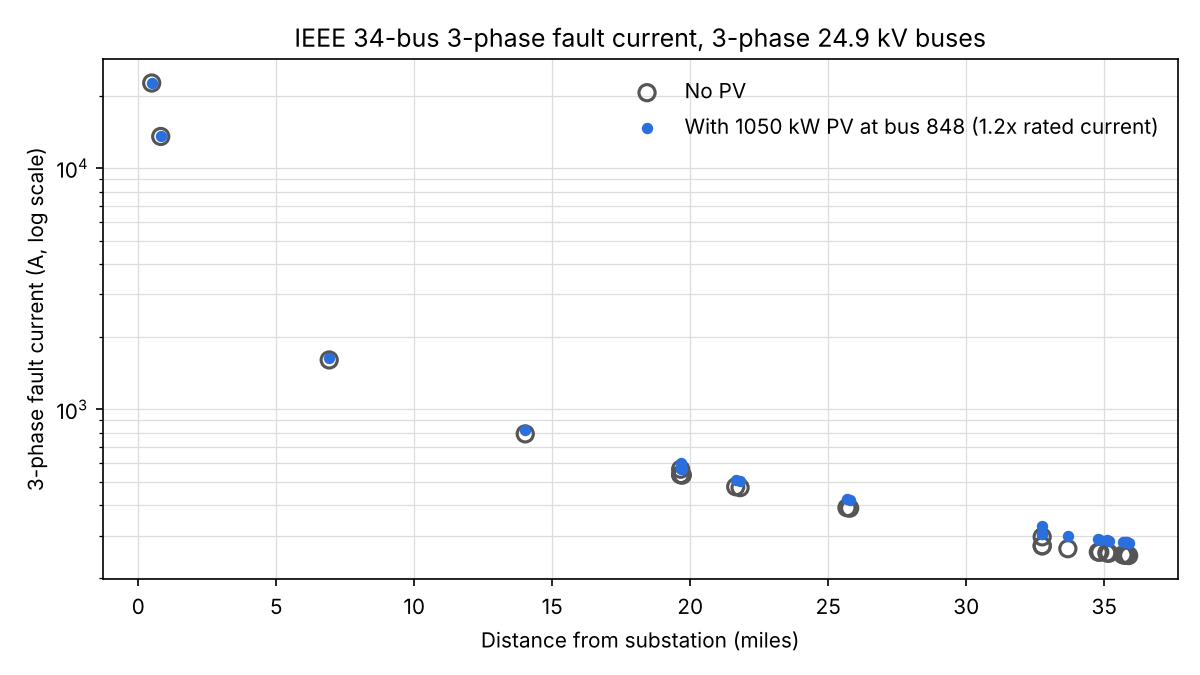
\includegraphics[width=0.85\textwidth]{figures/fig_step5_fault_current.png}
\caption{Three-phase fault current on three-phase \SI{24.9}{kV} buses, without PV and with 1{,}050\,kW PV at
bus 848 (log scale).}
\label{fig:fault}
\end{figure}

\begin{table}[H]
\centering
\small
\begin{tabular}{@{}lrrrcc@{}}
\toprule
Case & PV (kW) & Rated $I$ (A) & PV fault $I$ (A) & \% of $I_{sc}$ at 848 & 10\,\% / 15\,\% screens \\
\midrule
Unity PF & 800 & 20.8 & 24.9 & 10.1\,\% & Fail / Fail \\
Volt-var & 900 & 23.4 & 28.0 & 11.3\,\% & Fail / Fail \\
0.95 PF & 1{,}050 & 27.3 & 32.7 & 13.2\,\% & Fail / Fail \\
\bottomrule
\end{tabular}
\caption{Interconnection screens. 15\,\% of the \SI{1769}{kW} peak load is \SI{265}{kW}.}
\label{tab:screens}
\end{table}

\subsection{Discussion}
In absolute terms the PV adds little fault current: at most 33\,A, raising the end-of-line three-phase fault
current from \SI{248}{A} to \SI{281}{A} (+13\,\%). This is negligible for breaker and recloser duty. The 10\,\%
screen fails only because the feeder's end-of-line fault current is so low; a protection review should still
confirm that the substation relay detects end-of-line faults with PV infeed and that reclosing is coordinated
with the inverter's anti-islanding trip. The 15\,\% screen (265\,kW) is about one-third of the 800\,kW this study
found acceptable, which shows how conservative fast-track screens are on long feeders and why the detailed
study was worth doing.

% =====================================================================
\section{Problems Found and Lessons Learned}
\begin{enumerate}
  \item \textbf{Regulator taps are not unique.} The first comparison showed a 1.36\,\% voltage error. It was
        not a modeling error: OpenDSS had settled RG10 phase A two taps higher than IEEE's program. Matching taps
        before comparing networks reduced the error tenfold.
  \item \textbf{The IEEE base case is a peak-load case.} Its 1.05\,pu source already violates Range A at light
        load with no PV. Checking the no-PV case over the whole year before adding PV caught this, and the
        setpoint turned out to be the largest single lever on hosting capacity. Lowering it, however, moved the
        problem to undervoltage at bus 814 at heavy load (296\,h/yr): with an unregulated section at the head of
        the feeder, one fixed setpoint cannot meet both limits.
  \item \textbf{Round-off error.} An early version of the script reported the 0\,kW case as a failure at
        ``1.0500\,pu'': bus 800 sat a hair above 1.05\,pu because of round-off. A 0.0001\,pu tolerance fixed it.
  \item \textbf{Placeholder data.} OpenDSS gives every line a 400\,A rating unless told otherwise. Without real
        ampacities the thermal check would have been meaningless.
  \item \textbf{Single-phase buses in the fault screen.} The first version of the screen compared the
        three-phase PV with the fault current at single-phase bus 838. Restricting the comparison to three-phase
        buses gave the correct weakest bus (848).
  \item \textbf{OpenDSS changes the working directory.} After \texttt{compile}, relative paths point into the
        model folder; all scripts build absolute paths from the script's own location.
  \item \textbf{External services change.} The old PVWatts address (pvwatts.nrel.gov) stopped resolving after
        NREL was renamed the National Laboratory of the Rockies; the tool had moved to a new address.
        Saving the downloaded profile in the repository keeps the study reproducible.
  \item \textbf{Local control has local vision.} Volt-var could not see the problem bus because a regulator
        sat between them. Where the limit is upstream, fixed PF or utility-side regulation is more effective.
\end{enumerate}

% =====================================================================
\section{Limitations and Future Work}
\begin{itemize}
  \item \textbf{Fixed substation setpoint:} the 1.03\,pu source is held all year, which leaves bus 814 below
        0.95\,pu for 296\,h/yr at heavy load. A load-dependent LTC schedule would fix this but lower the hosting
        capacity; repeating the sweeps with such a schedule is the most important next step.
  \item \textbf{One location:} PV was studied only at bus 848. A hosting capacity map over all three-phase buses
        would show where PV fits best (PV upstream of RG10 would likely behave very differently).
  \item \textbf{One load shape for all loads:} real feeders mix residential and commercial customers.
  \item \textbf{Static regulator control:} hourly snapshots ignore regulator time delays and tap-count wear,
        which PV variability increases.
  \item \textbf{Assumed data:} line ampacities from standard tables; inverter fault current assumed at
        1.2 times rated.
  \item \textbf{Not studied:} flicker and rapid voltage change, protection coordination, anti-islanding,
        volt-watt control.
  \item \textbf{Planned extension:} a fast machine-learning surrogate model trained on these simulations to
        estimate hosting capacity without the full time-series run.
\end{itemize}

% =====================================================================
\section{Conclusion}
A validated OpenDSS model of the IEEE 34-bus feeder was built and driven from Python. It matched IEEE's
published bus voltages within 0.14\,\%. A full-year, hourly study found a PV hosting capacity at bus 848 of
800\,kW at unity power factor, 900\,kW with IEEE 1547-2018 volt-var and 1{,}050\,kW at a fixed 0.95 power
factor. In every case the limit was overvoltage at the end of the unregulated section, and a simple
$(PR-QX)/V^2$ estimate reproduced both the voltage slope and the benefit of each inverter mode. The
substation setpoint mattered more than any inverter setting, but a fixed 1.03\,pu setting trades light-load
overvoltage for heavy-load undervoltage at bus 814, so in practice the setpoint must follow the load. Fast-track screens would have allowed only a
third of the capacity the detailed study supports. The project showed in practice how regulators, reverse
power flow and local inverter control interact on a long rural feeder, and how a utility interconnection
study moves from model validation to time-series analysis, protection checks and screens.

% =====================================================================
\section*{References}
\addcontentsline{toc}{section}{References}
\begin{enumerate}[label={[\arabic*]}]
  \item IEEE PES Distribution Test Feeder Working Group, \emph{IEEE 34 Node Test Feeder}, data and power flow
        results. \url{https://cmte.ieee.org/pes-testfeeders/resources}
  \item IEEE Std 1547-2018, \emph{IEEE Standard for Interconnection and Interoperability of Distributed Energy
        Resources with Associated Electric Power Systems Interfaces}.
  \item ANSI C84.1, \emph{Electric Power Systems and Equipment --- Voltage Ratings (60 Hz)}.
  \item EPRI, OpenDSS 11.0.0.1 and IEEE test case files; DSS-Extensions, OpenDSSDirect.py 0.9.4.
  \item National Laboratory of the Rockies (formerly NREL), \emph{PVWatts Calculator V8}, NSRDB TMY data.
  \item W.\,H. Kersting, \emph{Distribution System Modeling and Analysis}, CRC Press.
  \item Arizona Administrative Code R14-2-2615, \emph{Screens}.
        \url{https://www.law.cornell.edu/regulations/arizona/Ariz-Admin-Code-SS-R14-2-2615}
  \item M.\,J. Reno and R.\,J. Broderick, ``Technical Evaluation of the 15\,\% of Peak Load PV Interconnection
        Screen,'' Sandia National Laboratories. \url{https://www.osti.gov/servlets/purl/1256260}
\end{enumerate}

% =====================================================================
\appendix
\section{Script Listings}
The complete repository is at \url{https://github.com/mhasan-ee/ieee34-hosting-capacity}. The two main
scripts are listed here.

\subsection{\texttt{hosting\_capacity.py}}
\lstinputlisting{code/hosting_capacity.py}

\subsection{\texttt{fault\_study.py}}
\lstinputlisting{code/fault_study.py}

\section{Running the Study}
\label{app:run}
In PowerShell, from the project folder:
\begin{lstlisting}[language=bash, numbers=none]
py -3.12 -m venv .venv
.venv\Scripts\Activate.ps1
pip install -r requirements.txt

python run_powerflow.py                       # Step 1
python compare_ieee.py                        # Step 2, OpenDSS taps
python compare_ieee.py ieee                   # Step 2, IEEE taps
python hosting_capacity.py                    # Step 3, unity PF, 1.03 pu source
python hosting_capacity.py 848 1.05           # Step 3, IEEE 1.05 pu source
python hosting_capacity.py 848 1.03 50 vv     # Step 4, volt-var
python hosting_capacity.py 848 1.03 50 pf95   # Step 4, 0.95 PF absorbing
python make_fig_step4.py
python fault_study.py                         # Step 5
python one_line.py                            # Step 6
python report_figures.py                      # extra report figures
python setpoint_check.py                      # substation setpoint trade-off
\end{lstlisting}
Each hosting capacity run takes about 20--50\,s on a laptop.

\section{Project Log}
\begin{table}[H]
\centering
\small
\begin{tabular}{@{}p{2.1cm}p{1.6cm}p{11.3cm}@{}}
\toprule
Date & Step & Result \\
\midrule
Nov 14, 2026 & 1 & Python 3.12 venv, OpenDSSDirect.py 0.9.4. Base case: 2047.0\,kW, 283.3\,kvar, losses 273.5\,kW, 25 iterations \\
Nov 14 & 2 & Validation: mean 0.58\,\% / max 1.36\,\% with auto taps; 0.06\,\% / 0.14\,\% with IEEE taps \\
Nov 14 & 3 & Profiles checked (8{,}760 h). 1.05\,pu source gives 1.0528\,pu at 814 with no PV; 1.03\,pu adopted. HC unity = 800\,kW \\
Nov 14--15 & 4 & Volt-var 900\,kW; 0.95 PF 1{,}050\,kW; 1.05\,pu source 100\,kW \\
Nov 15 & 5 & $I_{sc}$ at 848 = 247.8\,A; PV adds 24.9--32.7\,A (10.1--13.2\,\%); both screens fail \\
Nov 15 & 6--8 & One-line diagram from the model; README; public GitHub repository \\
Nov 15 & -- & Setpoint check: fixed 1.03\,pu puts bus 814 below 0.95\,pu for 296\,h/yr (14\,h at 1.05\,pu); trade-off documented \\
\bottomrule
\end{tabular}
\caption{Running log of the study.}
\end{table}

\end{document}
